\section{\label{sec:pertth}微扰论中的矩阵元}

我在图~\ref{fig:sqpdf_tree} 中展示涂抹非单态矩阵元的领头阶（即树图级）贡献。在图~\ref{fig:sqpdf_tree} 与图~\ref{fig:sqpdf1} 中，我采用如下约定：实线表示费米子传播子；双线是费米子流核；空心方块是任意流时 $\tau_1$ 处的流顶点；灰圈表示固定流时 $\tau$ 的费米子场；灰方块表示固定流时 $\tau$ 处的顶点；虚线是空间延展的 Wilson 线算符。
注意，在单圈微扰论中规范流核对涂抹非单态准分布没有贡献。树图级贡献为
\begin{align}
\hm^{(0)} = {} & \frac{1}{2p}\big\langle  \,p,s \,\big| \overline{\chi}(n;\tau)\gamma_\alpha\frac{\lambda^a}{2}\chi(0;\tau) \big|\, p,s \, \big\rangle \nonumber\\
= {} & \frac{1}{2p}e^{ip_zz} e^{-2p^2\tau}\overline{u}^s(p)\frac{\lambda^a}{2}\gamma_\alpha u^s(p),
\end{align}
其中为清晰起见我略去了矩阵元的宗量，并且我使用了
\begin{equation}
\chi(x;\tau) \big | \,p,s \,\big\rangle = e^{-p^2\tau}\psi(x)\big | \,p,s \,\big\rangle =e^{-p^2\tau}e^{ip\cdot x}u^s(p),
\end{equation}
以及反夸克的类似关系。

超出树图级，算符收到可写为
\begin{align}
\hm^{(\mathrm{s})}= {} & {\cal Z}_h \hm^{(0)} \nonumber\\
= {} & Z_h^{(1)}(\oz^2,\mu^2\tau) Z_\chi^{(1)}(\mu^2\tau) \big(Z_\psi^{(1)}\big)^{-1}\hm^{(0)}+{\cal O}(\alpha_s^2). \label{eq:matchrel}
\end{align}
的辐射修正。这里 $\alpha_s = g^2/(4\pi)$ 是重正化耦合常数，它在此阶等于裸耦合常数，且最自然地在标度 $\mu^2 = 1/r_\tau^2$ 下取值。图~\ref{fig:sqpdf1} 展示对修正参数 ${\cal Z}_h$ 有贡献的各个单圈图。图 (a) 至 (f) 对算符重正化参数 $Z_h$ 有贡献。波函数重正化 $Z_\psi$ 收到图 (g) 的贡献。额外费米子波函数重正化 $Z_\chi$ 收到图 (h)、(i)、(j) 的贡献，它通过环标费米子被自动移除。

算符重正化参数 $Z_h$ 的确定是本文的核心结果。两个波函数重正化参数已在别处出现（特别地，$Z_\chi$ 在文献 \cite{Luscher:2013cpa,Makino:2014taa} 中计算）；我为完备性并作为对我方法的检验而计算这些贡献，并把它们与 $Z_h$ 结合得到完整的单圈修正 ${\cal Z}_h$。我证明，在小流时与定域矢量流极限下，参数 ${\cal Z}_h$ 约化为文献 \cite{Makino:2014taa,Hieda:2016lly} 中的相应结果，这是对我结果的非平凡检验。延展算符存在良好定义的定域矢量流极限，这与例如无流时时 $\ms$ 方案下的延展算符 \cite{Constantinou:2017sej} 形成对照，是涂抹准分布的一个吸引人的特点。

我把下面的讨论分成两部分，从矩阵元紫外结构的解析研究开始。这足以提取 $Z_h^{(1)}$，且之所以可能，是因为我假设重正化标度远大于外部动量并把动量设为零 \cite{Ishikawa:2016znu}。图 (b)、(c)、(e)、(i) 与外部动量成正比，在此情形下为零。此外，其余积分本身大为简化并变得可以解析处理。我用维数正规化调节由此产生的红外发散，并证明这些发散在 $\ms$ 方案矩阵元与非零流时矩阵元的匹配程序中抵消。在讨论的第二部分（第~\ref{sec:numres} 节），我对外部动量、夸克质量与流时的函数关系数值求值所有九个依赖流时的图，以展示单圈微扰论下完整矩阵元的行为。


\subsection{顶点型图}

在单圈微扰论中，与扩展算符相联系的有三个非零的``顶点型''图，即图~\ref{fig:sqpdf1} 中的 (a)、(d)、(f)，以及四个``波函数型''图，即图~\ref{fig:sqpdf1} 中的 (g) 至 (j)。在有限 Wilson 线长度 $z$ 下，各图表现出如下紫外与共线行为：图 (a) 紫外有限而对数红外发散，而图 (d) 与 (f) 若无流时本应对数紫外发散，流时的存在使其紫外有限且红外有限。因此，我直接在四维计算图 (d) 与 (f)，但图 (a) 需要维数正规化来调节积分的红外行为；我取 $d = (4+2\eir)$。在零外部动量下，裸矩阵元的对称性与量纲保证最终结果只是 $\oz^2=z^2/r_\tau^2$ 的函数 \cite{Radyushkin:2016hsy}，尽管个别图还可能依赖 $\mu^2$、$z^2$ 与 $\tau$ 的无量纲组合。我不对任何中间结果的函数依赖施加约束，因此确立最终结果只依赖 $\oz^2$ 是对计算的有用交叉检验。

为说明计算，我考虑图 (a)。图 (d) 与 (f) 的计算过程非常类似。零外部动量下，该图对 $Z_h$ 的贡献为
\begin{equation}
Z^{\mathrm{(a)}} = C_F (-ig_0\gamma_\rho)\! \int_k \frac{e^{-\tau k^2}}{i\kslash}\gamma_\alpha e^{-ik\cdot n} \frac{e^{-\tau k^2}}{i\kslash}(-ig_0\gamma_\sigma)\frac{\delta_{\rho\sigma}}{k^2}.
\end{equation}
这里 $C_F = 4/3$ 是色因子；$g_0$ 是裸耦合；所有重复的 Lorentz 指标求和；并且我定义
\begin{equation}
\int_k = \mu^{4-d}\int \frac{\mathrm{d}^dk}{(2\pi)^d}.
\end{equation}

分子的 Lorentz 结构是直接的，对分母使用 Schwinger 表示后，该积分变为
\begin{align}\label{eq:hma}
Z_h^{\mathrm{(a)}} = {} &  g_0^2C_F \frac{\mu^{4-d}}{(2\pi)^d} \int_0^\infty\mathrm{d}\alpha\,\frac{\alpha}{2} \nonumber \\
& \times \int \mathrm{d}^dk\, N_\alpha(k,d)e^{-(2\tau+\alpha) k^2} e^{-ik\cdot n}.
\end{align}
在有限流时与空间间隔下，分子 $N(k,d)$ 依赖于原矩阵元中 Lorentz 结构的选择。引入平行与垂直于类空间隔的动量分量 $k_z$ 与 $k_\perp=(k_x,k_y,k_t)$，对 $\hm^{(s)}$ 中取 $\gamma_\alpha = \gamma_z$ 的选择（式~\eqref{eq:hdef}），该分子为
\begin{equation}
N(k,d) \equiv (2-d)(k_z^2-k_\perp^2)
\end{equation}
而其他选择下为
\begin{equation}
N(k,d) \equiv (2-d)\left(\displaystyle\frac{3-d}{d-1}k_\perp^2 - k_z^2\right).
\end{equation}

式~\eqref{eq:hma} 中的动量积分可通过对 $k_z$ 与 $k_\perp$ 分别积分完成，剩下的对 Schwinger 参数 $\alpha$ 的积分可以解析求出，分别给出
\begin{align}
Z_h^{\mathrm{(a)}} = {} & \left(\frac{g_0}{4\pi}\right)^2C_F\bigg[\frac{1}{\eir} -\gE-\log\left(\pi \mu^2z^2\right) +3\nonumber\\
{} - \frac{3}{\oz^4} & \Big(e^{-\oz^2}-1\Big)- \frac{1}{\oz^2} \left(4-e^{-\oz^2}\right)+\ei{-\oz^2}\bigg], \label{eq:hta1}
\end{align}
与
\begin{align}
Z_h^{\mathrm{(a)}} = {} &\left(\frac{g_0}{4\pi}\right)^2C_F \bigg[\frac{1}{\eir}-\gE-\log\left(\pi \mu^2z^2\right)+1\nonumber\\
&{} -\frac{1}{\oz^4}\Big(1-e^{-\oz^2}(1+\oz^2)\Big)+\ei{-\oz^2} \bigg], \label{eq:hta2}
\end{align}
这里 $\ei{z}$ 是指数积分
\begin{equation}
\ei{z} = -\int_{-z}^\infty \frac{e^{-t}}{t}\mathrm{d}t.
\end{equation}
正如预期，梯度流不影响该图的红外结构（附录给出无梯度流时的等价结果）。

我以类似方式处理其余的图 (d) 与 (f)，得到
\begin{align}
Z_h^\mathrm{(d)} = {} & 2 g_0^2C_F\frac{\pi^2}{(2\pi)^4}\int_0^\infty\mathrm{d}\alpha\,\frac{\alpha}{(\alpha+2\tau)^2}\nonumber \\
{} & \qquad \qquad\qquad\times \left(1-e^{-z^2/(4(\alpha+2\tau))}\right),\\
Z_h^\mathrm{(f)} = {} & g_0^2C_F \frac{\pi^{d/2}}{(2\pi)^4}\int_0^\infty\mathrm{d}\alpha\,\frac{1}{(\alpha+2\tau)^{3/2}} \nonumber \\
\times {} & \int_0^\infty\mathrm{d}\beta\frac{1}{\sqrt{\alpha+\beta+2\tau}}\left(e^{-z^2/(4(\alpha+\beta+2\tau))}-1\right).
\end{align}
结果为
\begin{align}
\!\!Z_h^\mathrm{(d)} = {} & -\left(\frac{g_0}{4\pi}\right)^2C_F \cdot2\bigg[1-\gE-\log\left(\oz^2\right)+\ei{-\oz^2} \nonumber \\
{} & \qquad  + \frac{1}{\oz^2}\left(e^{-\oz^2}-1\right)\bigg], \label{eq:htd}\\
\!\!
Z_h^\mathrm{(f)} = {} & \left(\frac{g_0}{4\pi}\right)^2C_F \cdot2\bigg[\gE+\log\left(\oz^2\right)- \ei{-\oz^2}  \nonumber \\
{} & \quad {-} 2\left(e^{-\oz^2}-1\right) -2\sqrt{\pi\oz^2}\erf{\sqrt{\oz^2}}\bigg],
\label{eq:htf}
\end{align}
其中 $\erf{z}$ 是误差函数
\begin{equation}
%\Gamma(a,z) = {} & \int_z^\infty t^{a-1}e^{-t}\mathrm{d}t,\\
\erf{z} = \frac{2}{\sqrt{\pi}}\int_0^z e^{-t^2}\mathrm{d}t.
\end{equation}
这一项是预期的幂次发散的单圈贡献，在 $\oz \gg 1$ 时随 Wilson 线长度线性增长。

\subsection{波函数型图}

``波函数型''图是图~\ref{fig:sqpdf1} 中的 (g)、(h)、(j)［图 (i) 与外部动量成正比］。图 (g) 的贡献就是标准的夸克波函数重正化，由于它不依赖流时，将在涂抹分布与 $\ms$ 分布的单圈匹配关系中严格抵消。
一般地，在零外部动量且不存在其他标度时，该图在维数正规化下为零，但通过引入一个分离标度来暴露紫外与红外发散是有益的，我在附录中更详细地讨论这一点。

依赖流时的图 (h) 与 (j) 的发散部分通过使用环标费米子移除，后者纳入了与有限流时费米子相联系的额外费米子重正化 $Z_\chi$。图 (h) 与 (j) 含有发生在任意流时 $\tau_i$ 的流顶点，必须从零到 $\tau$ 积分。这些图的贡献为
\begin{align}
Z_h^\mathrm{(h)} = {} & 2 g_0^2C_F\cdot 2\int_0^\tau \mathrm{d}\tau_1
\int_k \frac{e^{-2k^2\tau_1}}{k^2} \nonumber \\
= {} & \left(\frac{g_0}{4\pi}\right)^2  C_F \cdot 2\left[\frac{1}{\euv}
+1+\log\big(8\pi\mu^2\tau\big)\right], \label{eq:hth}\\
Z_h^\mathrm{(j)}{} & (\mu^2\tau) = {-} 2g_0^2C_F  d\int_0^\tau \mathrm{d}\tau_1\int_k\frac{e^{-2k^2\tau_1}}{k^2} \nonumber \\
= {} & -\left(\frac{g_0}{4\pi}\right)^2C_F \cdot 4\left[\frac{1}{\euv} +\frac{1}{2} + \log(8\pi\mu^2\tau)\right]\label{eq:htj},
\end{align}
其中我已包含因子 2 以计入相应的反夸克修正。这些贡献不依赖非定域算符结构并被 $Z_\chi$ 中的项抵消，最初在文献 \cite{Endo:2015iea} 中对定域夸克双线性算符计算。

\subsection{单圈重正化参数}

汇集这些结果，我得到参数 $Z_h$ 的单圈表达式
\begin{equation}
Z_h^{(1)} =   1 + \frac{\alpha_s}{3\pi}\Big[Z_h^\mathrm{(a)}+Z_h^\mathrm{(d)} +Z_h^\mathrm{(f)}+Z_h^\mathrm{(g)}+Z_h^\mathrm{(h)}+Z_h^\mathrm{(j)}\Big],
\end{equation}
即
\begin{align}
Z_h^{(1)} = & {} 1 + \frac{\alpha_s}{3\pi}\bigg[-\frac{3}{\euv}+3\gE+3\log\left(\oz^2\right) -3\operatorname{Ei}(-\oz^2)\nonumber\\
{}  -4&\sqrt{\pi\oz^2}\erf{\sqrt{\oz^2}} -3\log(8\pi\mu^2\tau)+a(\oz^2)\bigg],
\end{align}
其中对 $\gamma_\alpha = \gamma_z$，
\begin{equation}
a(\oz^2) =  5 + \frac{3}{\oz^4} \Big(1-e^{-\oz^2}\Big)- \frac{1}{\oz^2} \left(2+e^{-\oz^2}\right)-4e^{-\oz^2},
\end{equation}
而其他选择下
\begin{equation}
a(\oz^2) =  3 - \frac{1}{\oz^4} \Big(1-e^{-\oz^2}\Big)+ \frac{1}{\oz^2} \left(2-e^{-\oz^2}\right)-4e^{-\oz^2}.
\end{equation}
这些表达式是本工作的核心结果。

\subsubsection{渐近行为}
这些单圈表达式满足若干交叉检验，其基础是在 $\oz \ll1 $ 与 $\oz \gg 1$ 渐近区域（分别对应定域矢量流极限与小流时极限）预期的结构。

\paragraph{矢量流极限}原则上，与维数正规化的情形（见附录）不同，只要已用适当的调节子（如红外截断或外部动量）调节了红外发散，在夸克场间隔趋于零的 $z\to 0$ 极限下就不存在接触项 \cite{Constantinou:2017sej}。此时可以直接取 $\oz\to 0$ 极限。但这里我用维数正规化处理红外发散，它现在表现为对 $\mu^2z^2$ 的对数依赖，这使程序复杂化。最简单的做法是在各个被积函数层面考察 $\oz\ll 1$ 区域，此时发现 $Z_h^\mathrm{(d)}=Z_h^\mathrm{(f)}=0$，且
\begin{equation}
\lim_{\oz \to 0}Z_h^\mathrm{(a)} =  \left(\frac{g_0}{4\pi}\right)^2C_F \left[\frac{1}{\eir}+\frac{1}{2} - \log\left(8\pi\mu^2\tau\right)\right],
\end{equation}
与原矩阵元中 $\gamma_\alpha$ 矩阵的选择无关，如预期。

将此结果与图 (h)、(j) 的表达式（它们不依赖空间间隔 $z$，当然依赖流时 $\tau$）结合，我得到
\begin{equation}
\lim_{\oz \to 0}Z_h^{(1)} = \left(\frac{g_0}{4\pi}\right)^2C_F \left\{\frac{1}{2}+\frac{1}{\eir}-\frac{3}{\euv} + \log\left(8\pi\mu^2\tau\right)\right\}.\label{eq:hoztozero}
\end{equation}
如下一节所示，与 $Z_\psi$ 和 $Z_\chi$ 结合后，参数 $Z_h^{(1)}$ 约化为文献 \cite{Hieda:2016lly} 的定域矢量流结果，这是该计算的一个重要检验。

\paragraph{小流时极限}在小流时极限，可以预期各图约化为 $\ms$ 方案中得到的表达式。图 (a) 约化为
\begin{equation}
Z_h^{(a)}  \stackrel{\oz \gg 1}{\simeq}\left(\frac{g_0}{4\pi}\right)^2C_F \bigg[\frac{1}{\eir} + C^{(\infty)}_\alpha-\gE-\log(\pi\mu^2z^2) \bigg],
\end{equation}
其中 $C^{(\infty)}_z = 3$，$C^{(\infty)}_\perp = 1$。这些结果与 $\ms$ 方案表达式（式~\ref{eq:ha_dr}）完全一致。
取 $\oz \gg 1$，图 (d) 与 (f) 变为
\begin{align}
Z_h^\mathrm{(d)}\!\! \stackrel{\oz \gg 1}{\simeq} {} & \!\!\!{-}\left(\frac{g_0}{4\pi}\right)^2C_F 2\bigg[1-\gE-\log(\oz^2) \bigg],\\
Z_h^\mathrm{(f)}\!\! \stackrel{\oz \gg 1}{\simeq} {} & \!\!\!\left(\frac{g_0}{4\pi}\right)^2C_F 2\bigg[1+\gE+\log(\oz^2)  +\left(1-2\sqrt{\pi}\oz\right) \bigg].
\end{align}
图 (f) 中括号内的贡献是线性发散，在与维数正规化的计算比较之前必须将其减去。移除该贡献后，这两图之和为
\begin{equation}
\left(Z_h^\mathrm{(d)} +Z_h^\mathrm{(f)}\right)\stackrel{\oz \gg 1}{=} 4\left(\frac{g_0}{4\pi}\right)^2C_F,\label{eq:hoztoinfty}
\end{equation}
与式~\eqref{eq:hd_dr} 和 \eqref{eq:hf_dr} 之和一致。简言之，$Z_h$ 的小流时极限与在 $\ms$ 方案中直接计算的相应结果精确匹配，正如预期。


\subsection{单圈涂抹矩阵元}

现在可以把波函数重正化 $Z_\psi$ 与 $Z_\chi$ \cite{Luscher:2013cpa,Makino:2014taa} 与上一节 $Z_h$ 的结果结合起来，写出完整的单圈涂抹矩阵元 $\hm^{(\mathrm{s})}$。回忆式~\eqref{eq:matchrel}，单圈矩阵元为
$\hm^{(\mathrm{s})} = {\cal Z}_hh^{(0)}$，其中
\begin{align}
{\cal Z}_h^{(1)} = & {} 1 + \frac{\alpha_s}{3\pi}\bigg[3\log\left(\oz^2\right) +6\gE-3\log(4\pi)-\log(432)\nonumber \\
{} &  -3\operatorname{Ei}(-\oz^2) -4\sqrt{\pi\oz^2}\erf{\sqrt{\oz^2}}+a(\oz^2)\bigg]
\end{align}
且这里
\begin{align}
c(\oz^2) = {} & 3\left[3+\frac{1}{\oz^2}\left(e^{-\oz^2}-2\right)+\frac{1}{\oz^4}\left(1-e^{-\oz^2}\right)\right] ,  \label{eq:cmuz}\\
c(\oz^2) = {} & 7 +\frac{1}{\oz^2}\left(3e^{-\oz^2}-2\right) +\frac{1}{\oz^4}\left(e^{-\oz^2}- 1\right),\label{eq:cmuperp}
\end{align}
分别对应 $\gamma_\alpha = \gamma_z$ 与 $\gamma_\alpha = \gamma_\perp$。我注意到图 (a) 顶点修正中的红外发散与波函数重正化（图 (g)）中的红外发散已经抵消。这与 $\ms$ 方案中的红外行为（式~\eqref{eq:zhmsbar}）一致，并证明梯度流不改变准分布的红外行为。此外，只要使用环标费米子，总单圈结果就是紫外有限的（即 $\euv$ 中没有极点），正如非零流时所保证的。对数项以如下方式组合：所有对 $\mu$ 的依赖都被消去，只留下 $\log(\oz)$。Wilson 线自能（图 (f)）产生一个按 $z/\sqrt{\tau}$ 标度的线性发散，与量纲预期一致。在更高阶微扰论中，可以预期该发散按 $e^{-cz/\sqrt{\tau}}$ 的形式指数化。

我在图~\ref{fig:Zozplot} 中以紫色与蓝色曲线分别画出 ${\cal Z}_{\mathrm{sub}}^{(z)}(\oz^2)$ 与 ${\cal Z}_{\mathrm{sub}}^{(\perp)}(\oz^2) $ 作为 $\oz$ 的函数。我已移除线性发散（否则它将在 $\oz\simeq 2$ 附近占主导），如点划灰线所示，它展示包含线性发散的 ${\cal Z}^{(z)}(\oz^2)$，图例中记为 ${\cal Z}^{(z)}(\oz^2)$。我还以橙色虚线画出 $\oz \ll 1$ 与 $\oz \gg 1$ 区域的渐近行为。
\begin{figure}
\centering
\caption{重正化参数 ${\cal Z}_h^{\mathrm{sub}}$ 在 $\gamma_\alpha=\gamma_z$ 与 $\gamma_\alpha = \gamma_\perp$ 下作为 $\oz$ 的函数，其中上标``$\mathrm{sub}$''表示线性发散已被减除。点划灰线是包含 $\oz$ 线性发散的 ${\cal Z}_h$，图例中记为 ${\cal Z}_h^{\mathrm{div}}$。我还以橙色虚线画出式~\eqref{eq:veclimit} 与 \eqref{eq:zsmalltau} 给出的 $\oz \ll 1$ 与 $\oz \gg 1$ 渐近行为。}
\label{fig:Zozplot}
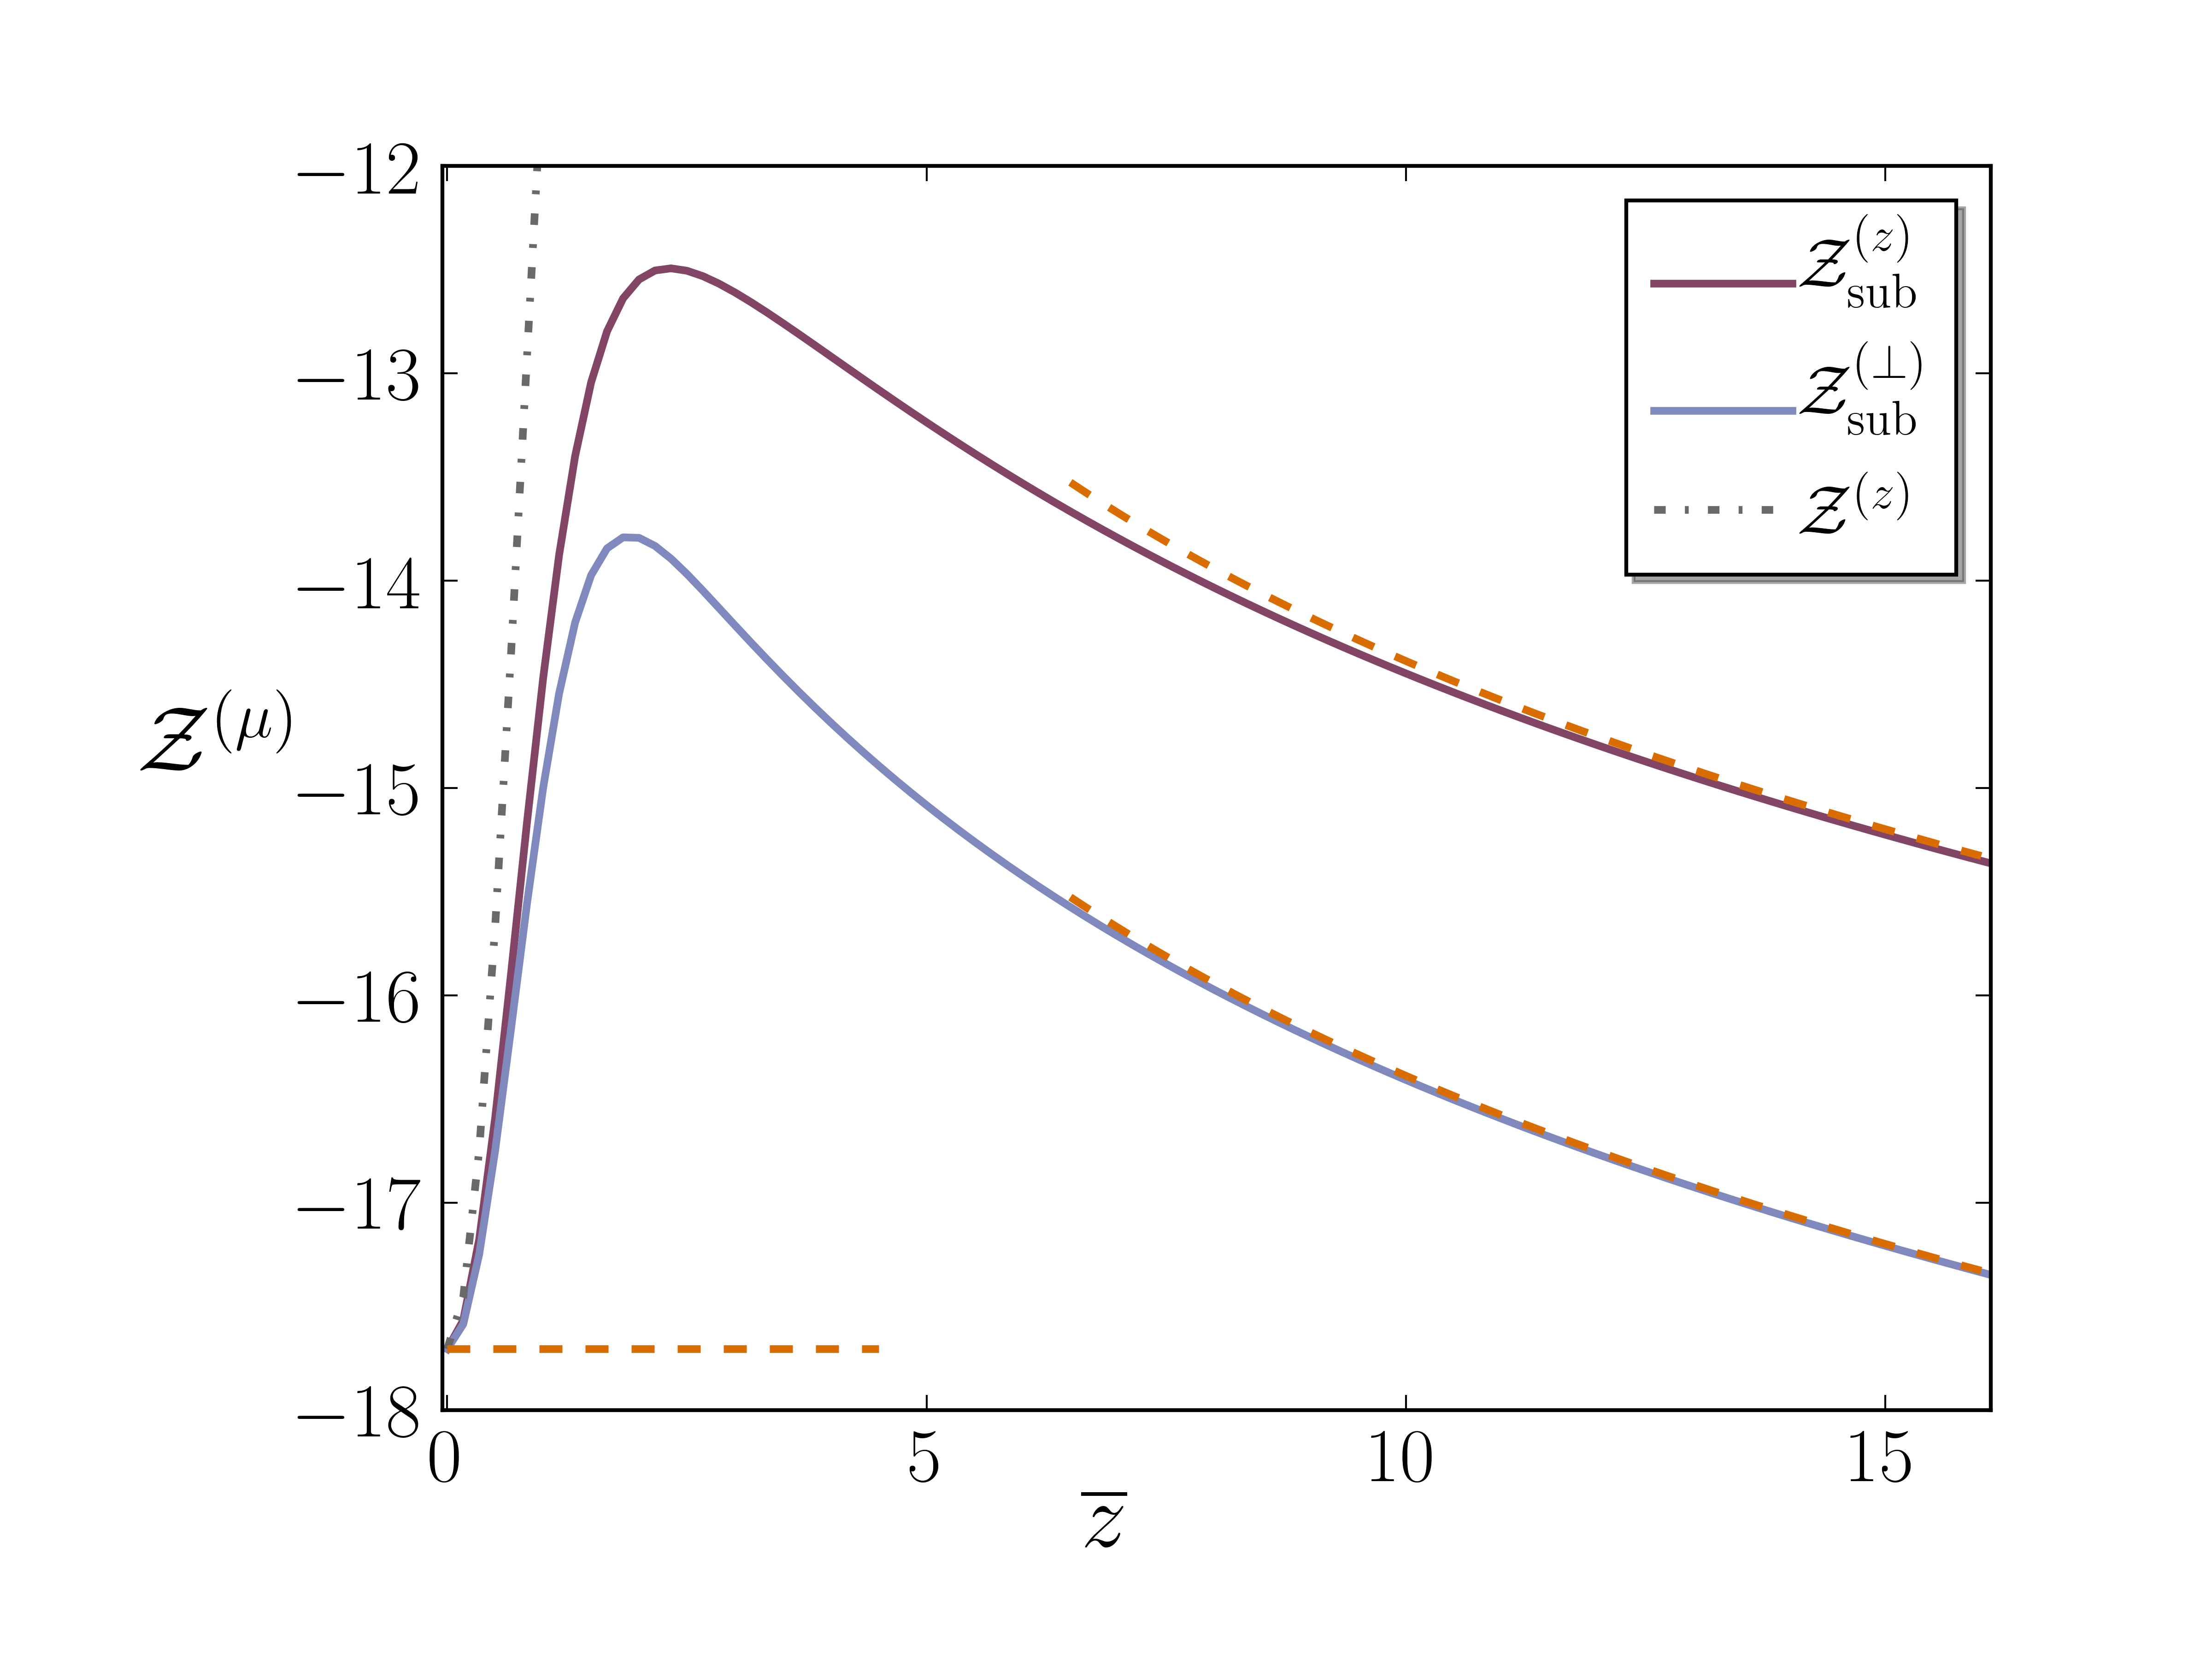
\includegraphics[width=0.47\textwidth,keepaspectratio]{images/zmu.png}
\end{figure}

\paragraph{矢量流极限}与维数正规化的矩阵元不同，夸克场空间间隔趋于零的 $\oz\to 0$ 极限是良好定义的，为
\begin{equation}\label{eq:veclimit}
\lim_{\oz\to0}{\cal Z}_h  = \frac{1}{2}-\log(432),
\end{equation}
它与 $\gamma_\alpha$ 的选择无关，并与文献 \cite{Hieda:2016lly} 的矢量流结果精确一致。该结果展示了由环标费米子构造的复合算符的一个特征：微扰修正是有限的（对守恒矢量流必须如此），但不一定为零（例如可与文献 \cite{Endo:2015iea} 定义的非单态轴矢流比较）。


\paragraph{小流时极限}相反，小流时展开给出
\begin{equation}\label{eq:zsmalltau}
{\cal Z}_h^{\mathrm{(sub)}} \stackrel{\oz\gg1}{\simeq} b - \gE - \log(432) - \log(\oz^2),
\end{equation}
其中 $\gamma_\alpha = \gamma_z$ 与 $\gamma_\alpha = \gamma_\perp$ 分别对应 $b = 9$ 与 $b=7$。在此区域，参数 ${\cal Z}_h^{\mathrm{sub}}(\oz^2)$ 仅对 $\oz$ 对数依赖，因此满足一个与通常重正化群方程类似的关系 \cite{Monahan:2015lha}：
\begin{equation}\label{eq:zsubRG}
\left[\frac{\mathrm{d}}{\mathrm{d}\log\oz^2} +\gamma_{\oz}\right]{\cal Z}_h^{\mathrm{sub}}(\oz^2) = 0.
\end{equation}
这里 $\gamma_{\oz} = \gamma_{\oz}^{(1)}\alpha_s+{\cal O}(\alpha_s^2)$（$\gamma_{\oz}^{(1)}=1$）类似于通常的反常量纲。超出单圈微扰论，完整的重正化群分析必须计入耦合常数 $\alpha_s(\mu)$ 的隐含标度依赖。重正化群轨迹于是成为二维空间 $(\oz,\mu)$ 中的一条路径，可通过把两个标度绑在一起（例如取 $\mu = 1/r_\tau$）来简化 \cite{Monahan:2015lha}。原则上，这可提供机会为矩阵元 $\hm^{(\mathrm{s})}(\oz^2)$ 构造非微扰的步标度（step-scaling）方法，把强子标度下的格点计算与一个高标度连接起来，在该高标度处与 $\ms$ 方案的匹配可以在没有显著微扰截断不确定度的情况下进行。然而，式~\eqref{eq:zsubRG} 只在小流时区域成立，由图~\ref{fig:Zozplot}，至少在单圈微扰论中该区域对应 $\oz \simeq 10$。在整个步标度程序中都强加这一约束对现有格点可能不可行，但与小流时预期的偏离相联系的系统不确定度可以非微扰地研究。


\subsection{坐标空间中的匹配}

有了完整的单圈涂抹准分布表达式，我就可以把结果与 $\ms$ 方案中重正化的矩阵元 $\hm^{\ms}(\mu^2z^2)$（见附录）匹配。写成
\begin{equation}
\hm^{\ms}(\mu^2z^2) = {\cal C}_h^{\mathrm{sub}}(\mu^2z^2,\oz^2)\hm^{(\mathrm{s})}(\oz^2),
\end{equation}
则匹配因子为
\begin{align}
%\!\!{\cal C}_h^{\mathrm{sub}}(\mu^2z^2,\oz^2){} &  = 1 +\frac{\alpha_s}{3\pi}\Big[3\overline{c}-c(\oz^2)+7\gE \nonumber\\
%\! +3\log(432) -{} & \ei{-\oz^2} +\log\left(\oz^2\right)+3\log\left(\mu^2z^2\right) \Big].\\
\!\!{\cal C}_h^{\mathrm{sub}}(\mu^2z^2,\oz^2){} &  = 1 +\frac{\alpha_s}{3\pi}\Big[a(\oz^2)-3\overline{c} -\log(432)\nonumber\\
 - 3\ei{-\oz^2} {} & -3\log\left(8\pi\mu^2t\right) -4\sqrt{\pi\oz^2}\erf{\sqrt{\oz^2}}\Big].
\end{align}
这里 $c(\oz^2)$ 由式~\eqref{eq:cmuz} 与 \eqref{eq:cmuperp} 给出，且 $\overline{c} =5/3$ 与 $\overline{c} =7/3$。一般地，线性发散将被非微扰地减除，我已从匹配关系中移除该贡献，由下标``$\mathrm{sub}$''标示。
零外部动量下，该匹配参数为实；在有限外部动量下（下一节讨论），匹配参数变为虚 \cite{Constantinou:2017sej}。
